\section{Interaction Analysis}

In figure \ref{Fig2} we plot conditional entropy of modality and
action for incoming/outgoing interactions constrained to the link
liked by atleast k friends.  Figure \ref{Fig2} shows that
\begin{itemize}
  \item Some interactions are more predictive than other. For
    eg. videos and photo interactions were found to be significantly
    more predictive than post and link interactions. Similarly,
    tagging action is often more predictive than commenting and
    liking.
  \item As noted by previous work~\cite{saez2011high}, we observe that
    outgoing interactions are more predictive than incoming
    interactions. Furthermore, the differentiation between
    predictiveness modalities and actions is more pronounced in
    outgoing interactions than in incoming interactions.
  \item It shows that the conditional entropy decreases as the number
    of friends liking the link increases.  It suggests that the
    discriminitivenes of interaction social affinity features
    increases as more friend like the item.
\end{itemize}


%%%%%%%%%%%%%%%%%%%%%%%%%%%%%%%%%%%%%%%%%%%%%%%%%%%%%%%%%%%%%%%%%%%%%%%%%%%
\begin{figure*}
\centering
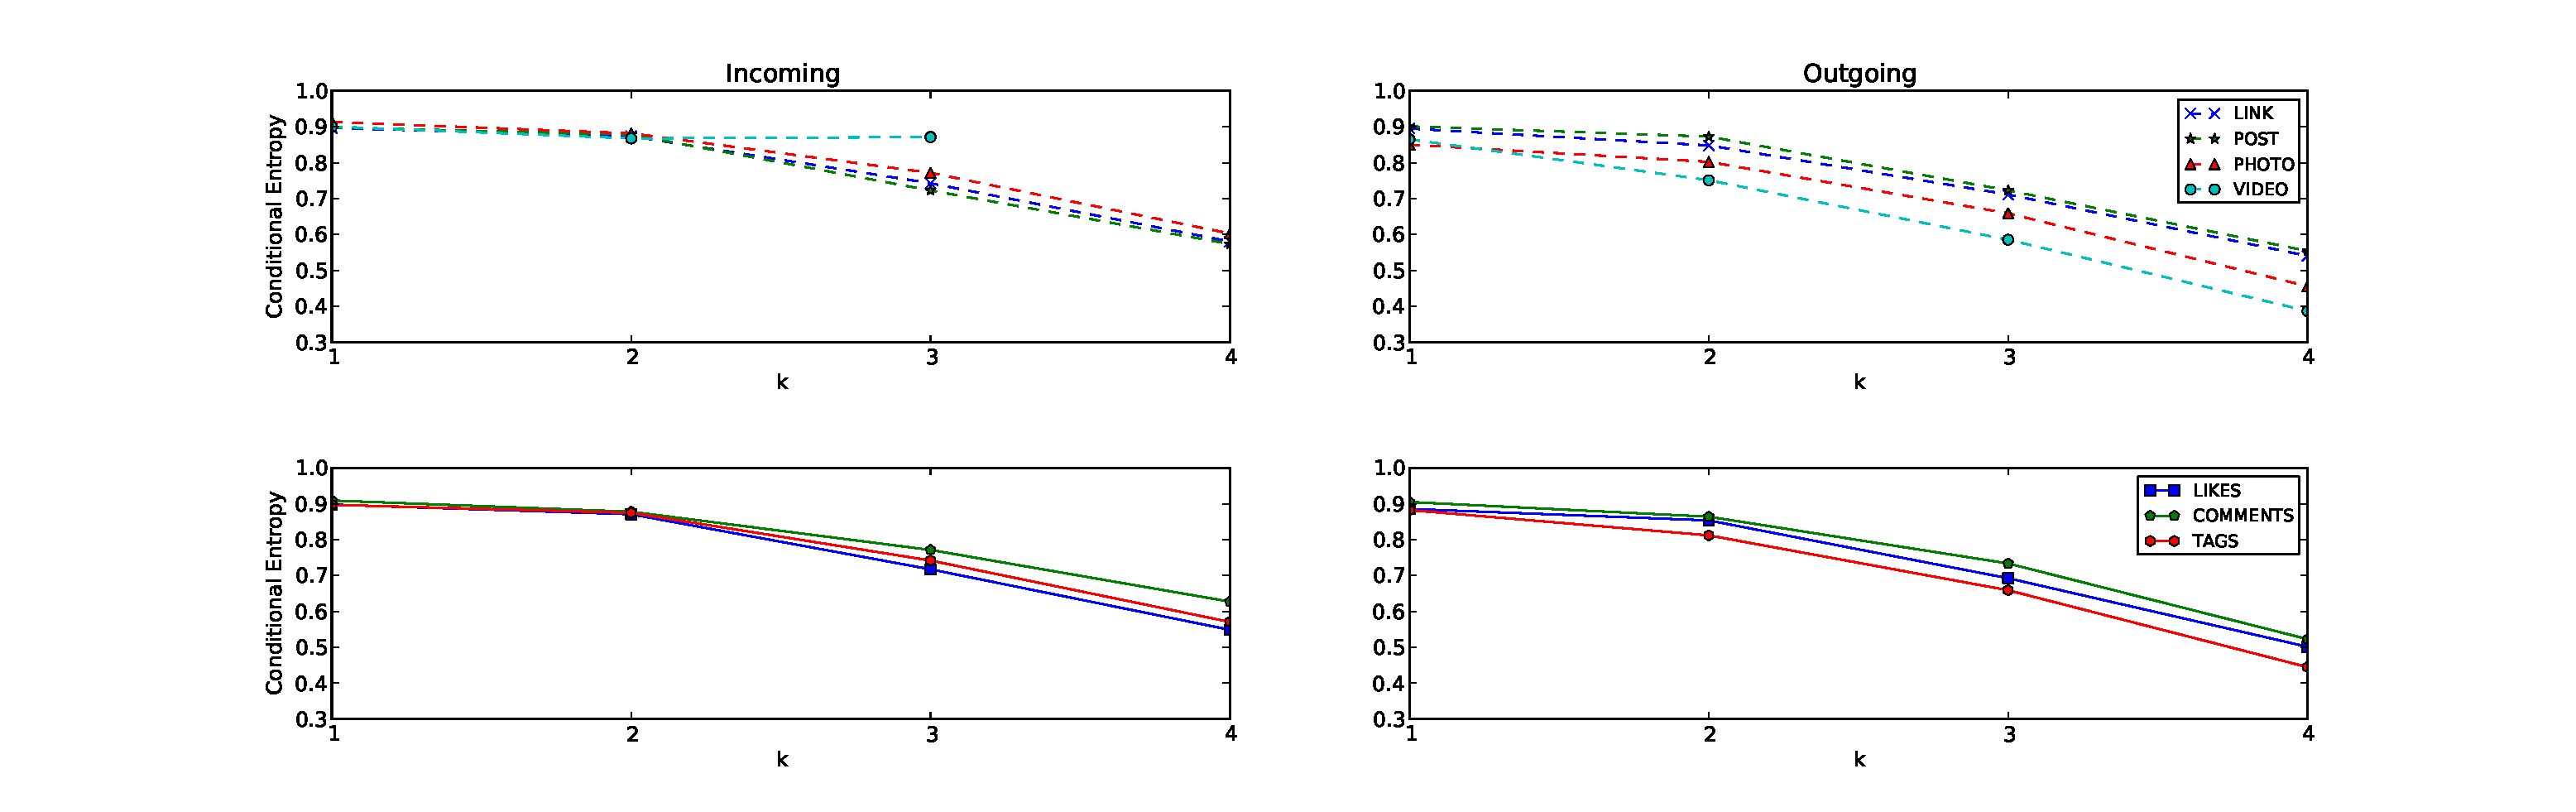
\includegraphics[width=160mm, height=40mm]{data/plots/vsk/ModalityActionsvsKFriends.eps}
\caption{Conditional Entropy  of modalities/activities for incoming/outgoing interactions vs item liked by atleast k friends}
\label{Fig2}
\end{figure*}
%%%%%%%%%%%%%%%%%%%%%%%%%%%%%%%%%%%%%%%%%%%%%%%%%%%%%%%%%%%%%%%%%%%%%%%%%%%
